\documentclass[10pt,letterpaper]{article}
\usepackage{fontspec}
\usepackage{amsmath,amssymb}
\usepackage{graphicx}
\usepackage{xcolor}
\usepackage{tcolorbox}
\tcbuselibrary{skins}
\usepackage{geometry}
\usepackage{booktabs}
\usepackage{colortbl}
\usepackage{fancyhdr}
\usepackage{titlesec}
\usepackage[shortlabels,inline]{enumitem}
\usepackage{tabularx}
\usepackage{array}
\usepackage{multicol}
\usepackage{tikz}

\setmainfont{Times New Roman}
\setsansfont{Arial}

\geometry{
    paperwidth=612.05pt,
    paperheight=720.05pt,
    top=20pt,
    headheight=14pt,
    headsep=12pt,
    bottom=28pt,
    footskip=12pt,
    left=36pt,
    right=36pt
}

\definecolor{stewartcyan}{RGB}{0, 118, 186}
\definecolor{stewartred}{RGB}{218, 41, 28}
\definecolor{stewarttableheader}{RGB}{210, 224, 238}
\definecolor{stewarttablehead}{RGB}{210, 224, 238}
\definecolor{tableblue}{RGB}{210, 224, 238}
\definecolor{stewartlightblue}{RGB}{235, 243, 250}
\definecolor{stewartblue}{RGB}{0, 118, 186}
\definecolor{stewartgray}{RGB}{120, 120, 120}
\definecolor{stewartlightgray}{RGB}{240, 240, 240}
\definecolor{stewartpurple}{RGB}{85, 30, 95}
\definecolor{stewartpurplebg}{RGB}{243, 238, 245}
\definecolor{stewartpurpletext}{RGB}{85, 30, 95}
\definecolor{darkgray}{RGB}{40, 40, 40}

\pagestyle{fancy}
\fancyhf{}
\renewcommand{\headrulewidth}{0pt}

\providecommand{\makecell}[2][c]{\begin{tabular}[#1]{@{}c@{}}#2\end{tabular}}
\providecommand{\faDesktop}{\textbf{[Máy tính]}}
\providecommand{\casicon}{\textbf{\textsf{[CAS]}}}
\providecommand{\ticon}{\textbf{\textsf{[T]}}}
\providecommand{\captionof}[2]{\par\vspace{2pt}{\small\textbf{#1}: #2}\par}
\NewDocumentEnvironment{tasks}{o d()}{\begin{enumerate}}{\end{enumerate}}
\providecommand{\task}{\item}
\newenvironment{redframebox}{\begin{definitionbox}}{\end{definitionbox}}

\newtcolorbox{definitionbox}{
    colback=white,
    colframe=stewartred,
    arc=0mm,
    boxrule=0.9pt,
    left=3.5mm, right=3.5mm, top=3mm, bottom=3mm
}

\begin{document}

\begin{document}

\fancyhead[L]{}
\fancyhead[R]{}

\noindent
\begin{minipage}[t]{0.26\textwidth}
    \vspace*{0.25cm}%
    {\color{stewartcyan}%
    \rule{\linewidth}{0.6pt}\vspace{3pt}\par
    \rule{\linewidth}{0.6pt}\vspace{3pt}\par
    \rule{\linewidth}{0.6pt}\vspace{3pt}\par
    \rule{\linewidth}{0.6pt}\par
    }
\end{minipage}%
\hfill
\begin{minipage}[t]{0.71\textwidth}
    \vspace*{0pt}%
    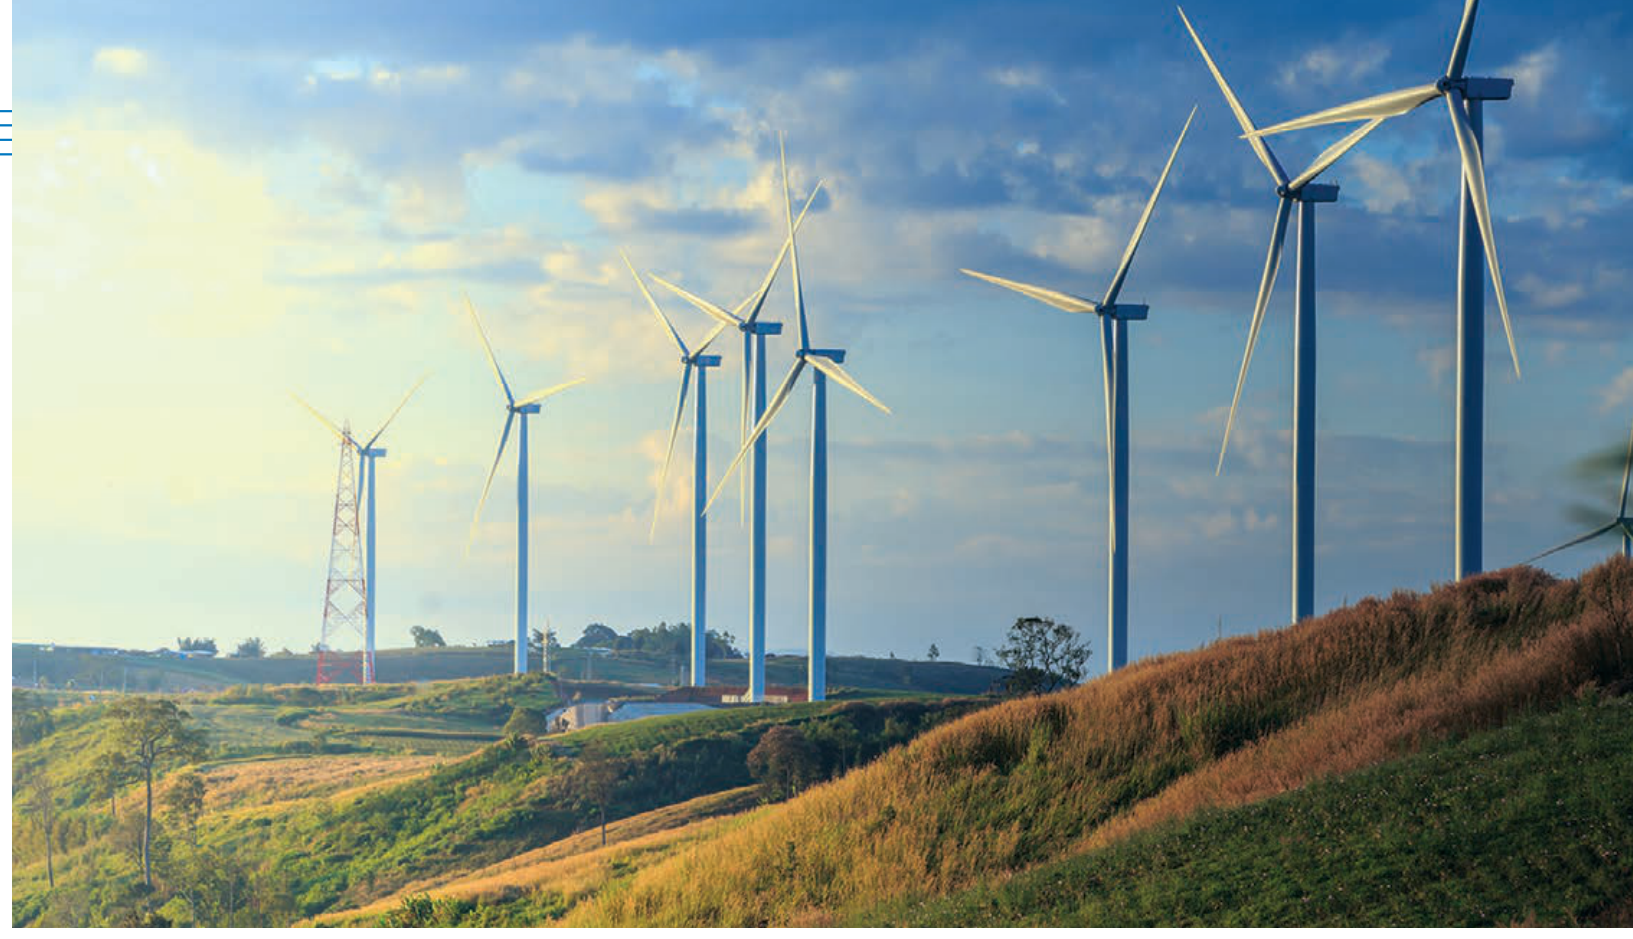
\includegraphics[width=\linewidth,height=8.3cm]{images/p0042_fig1.png}\par
    \vspace{0.15cm}
    {\fontsize{8.5pt}{11pt}\selectfont\sffamily Công suất điện do một tuabin gió tạo ra có thể được ước tính bằng một hàm số toán học kết hợp nhiều yếu tố. Chúng ta sẽ khám phá hàm số này trong Bài tập 1.2.25 và xác định công suất phát dự kiến của một tuabin cụ thể ứng với các tốc độ gió khác nhau.\par}
    \vspace{1.5pt}
    {\scriptsize\sffamily\color{black!70}chaiviewfinder / Shutterstock.com\par}
\end{minipage}

\vspace{0.7cm}

\noindent
\begin{minipage}[t]{0.26\textwidth}
    \vspace*{0.6cm}%
    \begin{flushright}
        {\fontsize{92}{92}\selectfont\sffamily\bfseries\color{stewartcyan}1\hspace{0.2cm}}
    \end{flushright}
\end{minipage}%
\hfill
\begin{minipage}[t]{0.71\textwidth}
    \vspace*{0pt}%
    \noindent
    \smash{\color{stewartcyan}\rule[-10.2cm]{1.5pt}{11.5cm}}\hspace{0.45cm}%
    \parbox[t]{\dimexpr\linewidth-1.5pt-0.45cm\relax}{%
        \vspace*{0.7cm}%
        {\fontsize{32}{38}\selectfont\sffamily\bfseries Hàm số và Mô hình\par}
        
        \vspace{0.75cm}
        \noindent
        \textbf{CÁC ĐỐI TƯỢNG CƠ BẢN MÀ CHÚNG TA} làm việc trong giải tích là các hàm số. Chương này chuẩn bị nền tảng cho giải tích bằng cách thảo luận về các ý tưởng cơ bản liên quan đến hàm số, đồ thị của chúng, cùng các phương pháp biến đổi và kết hợp hàm số. Chúng tôi nhấn mạnh rằng một hàm số có thể được biểu diễn theo nhiều cách khác nhau: bằng một phương trình, trong một bảng số liệu, qua một đồ thị, hoặc bằng lời. Chúng ta sẽ tìm hiểu các dạng hàm số chính xuất hiện trong giải tích và mô tả quá trình sử dụng các hàm số này làm mô hình toán học cho các hiện tượng trong thế giới thực.
    }
\end{minipage}

\vfill
\begin{flushright}
    {\fontsize{10}{12}\selectfont\sffamily\bfseries 7}
\end{flushright}

\end{document}
